\documentclass[border=10pt]{standalone}
\usepackage{tikz}
\usetikzlibrary{shapes, arrows.meta, positioning, fit, backgrounds}

\definecolor{hostblue}{HTML}{4A90D9}
\definecolor{espsoft}{HTML}{4A904A}
\definecolor{actred}{HTML}{D94A4A}

\tikzset{
    box/.style={rectangle, draw, fill=white, minimum width=1.8cm, minimum height=0.7cm, align=center, font=\small},
    group/.style={rectangle, draw, dashed, thick, inner sep=8pt},
    arr/.style={-{Stealth[length=2mm]}, thick},
    arrlab/.style={font=\scriptsize, fill=white, inner sep=1pt},
}

\begin{document}
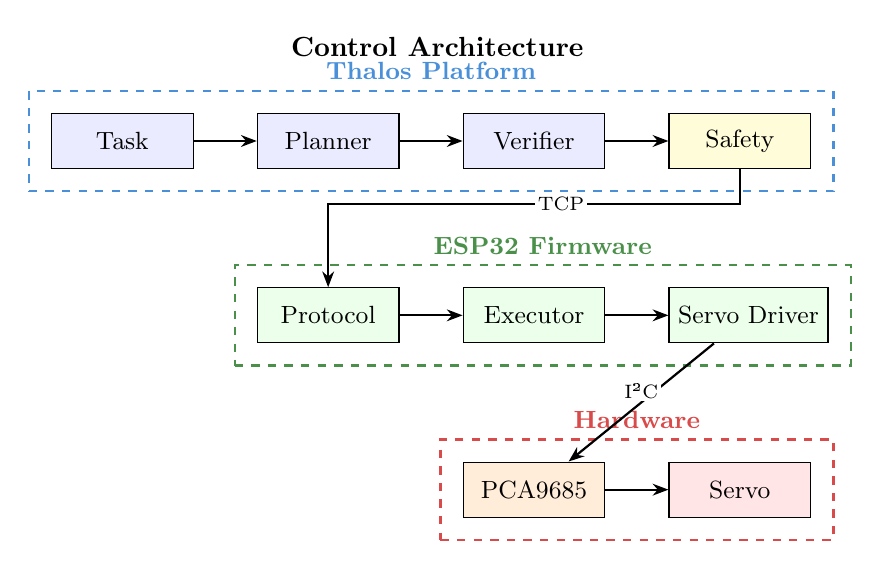
\begin{tikzpicture}[node distance=0.6cm and 0.8cm]

\node[font=\bfseries] at (4, 0.2) {Control Architecture};

% ── Thalos Platform ──
\node[box, fill=blue!8] (task) at (0, -1) {Task};
\node[box, fill=blue!8, right=of task] (plan) {Planner};
\node[box, fill=blue!8, right=of plan] (ver) {Verifier};
\node[box, fill=yellow!15, right=of ver] (safe) {Safety};

% Group: Thalos
\node[group, draw=hostblue, fit=(task) (plan) (ver) (safe), label={[font=\small\bfseries, hostblue]above:Thalos Platform}] {};

% ── ESP32 Firmware ──
\node[box, fill=green!8, below=1.5cm of plan] (proto) {Protocol};
\node[box, fill=green!8, right=of proto] (exec) {Executor};
\node[box, fill=green!8, right=of exec] (drv) {Servo Driver};

% Group: Firmware
\node[group, draw=espsoft, fit=(proto) (exec) (drv), label={[font=\small\bfseries, espsoft]above:ESP32 Firmware}] {};

% ── Hardware ──
\node[box, fill=orange!15, below=1.5cm of exec] (pca) {PCA9685};
\node[box, fill=red!10, right=of pca] (servo) {Servo};

% Group: Hardware
\node[group, draw=actred, fit=(pca) (servo), label={[font=\small\bfseries, actred]above:Hardware}] {};

% ── Connections ──
\draw[arr] (task) -- (plan);
\draw[arr] (plan) -- (ver);
\draw[arr] (ver) -- (safe);

\draw[arr] (safe) -- ++(0,-0.8) -| node[arrlab, pos=0.25, right] {TCP} (proto);

\draw[arr] (proto) -- (exec);
\draw[arr] (exec) -- (drv);

\draw[arr] (drv) -- (pca) node[arrlab, midway, above] {I²C};
\draw[arr] (pca) -- (servo);

\end{tikzpicture}
\end{document}
